\documentclass[11pt]{article}
\usepackage[a4paper,margin=2.4cm]{geometry}
\usepackage{booktabs,graphicx,amsmath,amssymb,hyperref,xcolor}
\hypersetup{colorlinks,linkcolor=blue!50!black,citecolor=blue!50!black,urlcolor=blue!50!black}
\usepackage[numbers,sort&compress]{natbib}

\title{Same Setting, Different Verdict:\\
\large How the Way a Terraform Value Is Written Changes What Security Scanners Report}
\author{Mithil Nagabathula\\University of East London\\\texttt{mithilnishu2000@gmail.com}}
\date{October 2026}

\begin{document}
\maketitle

\begin{abstract}
Infrastructure-as-code security scanners are commonly run as pipeline gates, and teams trust a clean result. We test two widely used
open-source scanners, Checkov and Semgrep's Terraform rules, with a mutation corpus: 24 security-relevant AWS settings, each written
secure and insecure in seven common Terraform idioms (a literal, a variable default, a \texttt{terraform.tfvars} file, a local value,
a conditional, a local module and an omitted attribute), giving 312 cases with known ground truth. Both scanners were perfect on
literals. Checkov resolved every indirection for 20 of the 21 settings it covers, but missed a \texttt{null} passed through a variable
for SNS encryption and flagged three of four omitted settings whose provider default is secure, including SQS queues that AWS has
encrypted by default since 2022. Semgrep resolved variable defaults and locals, but for values it could not see (tfvars, conditionals,
modules) its verdict was decided by the rule's polarity rather than the configuration: rules that require a secure literal flagged
secure and insecure cases alike (false-positive rate 0.79), and rules that look for an insecure literal missed them. On 53 real
projects (2{,}179 files), the scanners agreed on 7 of 63 resource-level findings in the categories both cover; all 18 of Checkov's SQS
encryption findings concerned queues relying on the default encryption. A clean scan therefore depends on code style as much as on
configuration. We release the corpus as a regression suite.
\end{abstract}

\section{Introduction}
Infrastructure as code lets teams review and test cloud configuration like software \cite{rahman2019mapping}, and static scanners turn
known misconfigurations into automated checks \cite{rahman2019seven,saavedra2022glitch}. In practice a scanner's result often gates a
merge. That makes two questions important: when a scanner passes a configuration, is it secure, and when it fails one, is it insecure?

Terraform offers many ways to express the same value. A setting can be a literal, a variable with a default, a value supplied in a
\texttt{terraform.tfvars} file, a local, a conditional on a feature flag, an input to a module, or left out so the provider default
applies. Real modules use these idioms constantly; the popular \texttt{terraform-aws-modules} expose almost every setting as a
variable \cite{tfawsmodules}. A scanner that only reasons about literals will be right on toy examples and unpredictable on real code.

We borrow the idea of mutation testing \cite{jia2011mutation}: hold the security meaning fixed, vary the syntax, and see whether the
verdict changes. Contributions:
\begin{itemize}
  \item a 312-case corpus with ground truth by construction, covering 24 AWS settings and seven idioms;
  \item a differential method that maps each scanner's rules to each setting automatically, avoiding hand-built rule mappings;
  \item measurements of recall and false positives per idiom for Checkov \cite{checkov} and Semgrep \cite{semgrep}, and an
        agreement study on 53 public projects.
\end{itemize}

\section{Method}
\subsection{Mutation corpus}
Each of the 24 categories is a single AWS resource with one security-relevant setting whose value is a plain HCL expression, for
example \texttt{storage\_encrypted} on \texttt{aws\_db\_instance}, \texttt{http\_tokens} in the EC2 metadata options, or the CIDR list on
an SSH ingress rule. Settings span encryption at rest and in transit, network exposure, identity, logging, resilience, key management
and supply chain. For each category we write a secure and an insecure value, and place it in six idioms:
\emph{literal}; \emph{variable default}; \emph{tfvars} (a variable without default, set in \texttt{terraform.tfvars});
\emph{local}; \emph{conditional} (\texttt{var.production ? value : other}, with \texttt{production} defaulting to true); and
\emph{module} (the resource inside \texttt{./modules/app}, with the value passed as an input). A seventh idiom, \emph{omitted}, drops the
attribute; its ground truth is the provider default, which is insecure for 20 categories and secure for four (RDS and Redshift public
access, the SSH CIDR, and SQS encryption, which AWS has applied by default since 2022 \cite{awssqssse}). This gives 312 cases.

\subsection{Scanners and rule mapping}
We ran Checkov 3.3.29 on each case directory with its default command line, as a CI job would, and Semgrep 1.181.0 with the Terraform
rules from the public \texttt{semgrep-rules} repository. To decide which rules belong to a category without a hand-built mapping, we
take the rules that fire on the insecure literal but not on the secure literal. A scanner \emph{covers} a category if this set is
non-empty. A case is \emph{flagged} if any of the category's rules fires on it. Checkov covered 21 categories and Semgrep 14; both
covered 12, and neither covered OpenSearch node-to-node encryption with the attribute we used.

\subsection{Real corpus}
We scanned 52 projects from \texttt{terraform-aws-modules} (each with its examples) and TerraGoat \cite{terragoat}, 2{,}179
\texttt{.tf} files. Findings were attributed to resources (Semgrep by the line of the match, Checkov by its resource address) and to
categories using the mapping above, and compared on the categories both scanners cover.

\section{Results}
\begin{table*}[t]
\centering
\caption{Recall on insecure cases and false-positive rate on secure cases, by how the security setting is written, over the categories each scanner covers (21 for Checkov, 14 for Semgrep). Omitted settings are counted as insecure or secure according to the provider default.}
\label{tab:idioms}
\small
\begin{tabular}{lrrrr}
\toprule
Setting written as & Checkov recall & Checkov FPR & Semgrep recall & Semgrep FPR \\
\midrule
Literal value & 1.00 (21/21) & 0.00 (0/21) & 1.00 (14/14) & 0.00 (0/14) \\
Variable default & 0.95 (20/21) & 0.00 (0/21) & 0.93 (13/14) & 0.00 (0/14) \\
terraform.tfvars & 0.95 (20/21) & 0.00 (0/21) & 0.79 (11/14) & 0.79 (11/14) \\
Local value & 0.95 (20/21) & 0.00 (0/21) & 0.93 (13/14) & 0.00 (0/14) \\
Conditional & 0.95 (20/21) & 0.00 (0/21) & 0.79 (11/14) & 0.79 (11/14) \\
Local module & 0.95 (20/21) & 0.00 (0/21) & 0.79 (11/14) & 0.79 (11/14) \\
Omitted (default) & 1.00 (17/17) & 0.75 (3/4) & 1.00 (10/10) & 0.25 (1/4) \\
\bottomrule
\end{tabular}
\end{table*}


\paragraph{Literals are easy.} Both scanners flagged every insecure literal and no secure literal in the categories they cover
(Table~\ref{tab:idioms}).

\paragraph{Checkov resolves indirection, with one null-handling gap.} Checkov evaluates variables, \texttt{terraform.tfvars},
locals, conditionals and local modules, and its verdict was unchanged across those idioms for 20 of 21 categories. The exception was
SNS encryption: the insecure value is \texttt{null}, and when that \texttt{null} arrived through a variable, local, conditional or module,
Checkov treated the attribute as set and passed it. Terraform treats an attribute set to \texttt{null} as omitted, so these
configurations create unencrypted topics.

\paragraph{Semgrep's verdict on unresolved values follows rule polarity.} Semgrep propagated variable defaults and locals for most
rules. For values it cannot see (tfvars, conditionals, modules) the result depended on how each rule was written. Rules phrased as
``flag unless the attribute is the secure literal'' flagged secure and insecure cases alike, producing both the 0.79 recall and the
0.79 false-positive rate in Table~\ref{tab:idioms}. Rules phrased as ``flag if the attribute is the insecure literal'' (RDS public
access, public-read ACLs, SSH from \texttt{0.0.0.0/0}) passed every unresolved case, secure or not. For the SSH rule this extended to
variable defaults and locals. Figure~\ref{fig:heat} shows the pattern per category.

\begin{figure}[t]
  \centering
  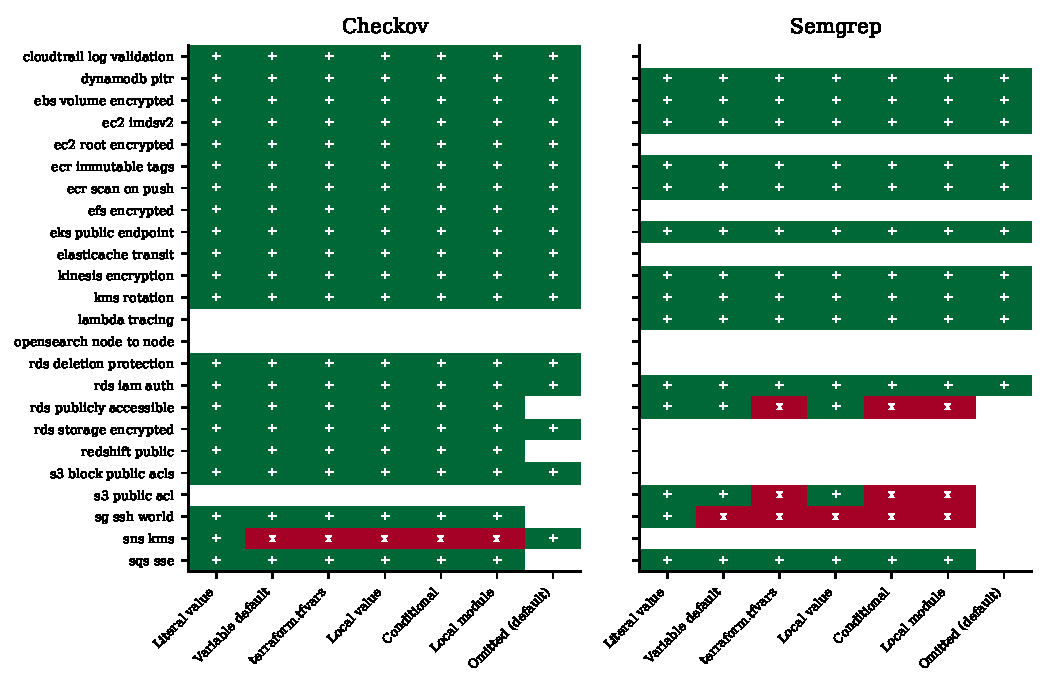
\includegraphics[width=\linewidth]{figures/heatmap.pdf}
  \caption{Insecure cases flagged (green, +) or missed (red, x) by category and idiom. Blank rows are categories a scanner does not cover; blank cells in the last column are settings whose default is secure.}
  \label{fig:heat}
\end{figure}

\paragraph{Omitted settings and outdated defaults.} Both scanners treated an omitted SQS encryption setting as insecure, although AWS has
encrypted new queues by default since 2022. Checkov also flagged an omitted Redshift public-access setting, whose default in current
versions of the AWS provider is private, and an SSH ingress rule with no source CIDR, which admits no traffic. These are false positives
that teams learn to suppress, and suppressions outlive the reason for them.

\paragraph{Real projects.} Checkov reported 2{,}255 failed checks across the 53 projects and Semgrep 281; Semgrep reported nothing at
all for 26 projects. On the 12 categories both cover, 63 resource-level findings were raised: 7 by both, 56 by Checkov only and none by
Semgrep only. The \texttt{terraform-aws-modules} set nearly every value through variables, which is exactly where Semgrep's rules stop
reasoning. All 18 of Checkov's SQS encryption findings were on queues that set no encryption attribute and therefore receive the
default SSE-SQS encryption.

\section{Discussion}
\paragraph{For teams.} A passing scan on modular Terraform says more about code style than about configuration when the scanner does
not evaluate expressions. Teams should know which of their scanners evaluate variables and modules, run scanners on the planned
configuration (for example, \texttt{terraform show -json} of a plan) where possible, and review suppressions when provider defaults
change.

\paragraph{For tool authors.} (1) When a value cannot be resolved, report \emph{unknown} rather than silently passing or failing; the
polarity effect is invisible to users. (2) Treat an explicit \texttt{null} as omitted. (3) Tie rules about defaults to provider
versions. (4) Use idiom-mutation suites like ours as regression tests; the corpus is small enough to run in CI.

\paragraph{Limitations.} Only two scanners were tested; others (Trivy, KICS, Terrascan) could not be installed in our environment and
should be added. We tested one setting per resource and AWS only. Ground truth for omitted values depends on provider and service
defaults at the time of writing. Rule mapping by differential firing can miss rules that fire on both literals; the corpus comparison
is limited to categories in the mutation corpus.

\section{Conclusion}
Holding the security meaning of a Terraform configuration fixed and changing only how a value is written changed scanner verdicts.
Checkov was robust to indirection apart from \texttt{null} values and outdated defaults; Semgrep's verdicts on indirect values were set by
rule polarity. On real modular code the two scanners rarely agreed. The idiom-mutation corpus is released for others to test their
tools.

\paragraph{Reproducibility.} Code, the mutation corpus and results will be released at
\newline\url{https://github.com/mithil2k2000-tech/iac-scanner-idioms}.

\paragraph{Use of AI tools.} An AI assistant (Claude, Anthropic) helped write experiment code and draft text. The author designed the
study questions, reviewed the code and results, and takes responsibility for the content.

\bibliographystyle{plainnat}
\bibliography{refs}
\end{document}
